\documentclass[12pt,a4paper]{article}

\usepackage[margin=2.5cm]{geometry}
\usepackage{amsmath,amssymb,amsthm}
\usepackage{mathtools}
\usepackage{graphicx}
\usepackage{booktabs}
\usepackage{hyperref}
\usepackage{natbib}
\usepackage{algorithm}
\usepackage{algpseudocode}
\usepackage{caption}
\usepackage{subcaption}
\usepackage{microtype}
\usepackage{setspace}
\usepackage{xcolor}

\singlespacing

% Theorem-like environments
\newtheorem{remark}{Remark}

% Shorthand macros
\newcommand{\D}{\mathcal{D}}
\newcommand{\N}{\mathcal{N}}
\newcommand{\E}{\mathbb{E}}
\newcommand{\R}{\mathbb{R}}
\newcommand{\pt}{\tilde{p}}
\newcommand{\KL}{\mathrm{KL}}
\newcommand{\ELBO}{\mathcal{L}}
\newcommand{\lam}{\lambda}
\newcommand{\sig}{\sigma}

\title{%
  \textbf{Bayesian Approximate Inference: \\
  Metropolis-Hastings MCMC and Mean-Field\\
  Stochastic Gradient Variational Inference}\\[0.5em]
  \large ESTR2020 Course Project Report
}
\author{Group XX}
\date{May 2026}

\begin{document}

\maketitle
\tableofcontents
\newpage

% ============================================================
\section{Abstract}
% ============================================================

This report presents a rigorous mathematical treatment and empirical evaluation
of two classes of approximate Bayesian inference methods applied to a model
with an analytically intractable posterior $p(\theta \mid \D)$.
Because the marginal likelihood involves a high-dimensional integral that cannot
be computed in closed form, exact posterior predictive computation $p(x^* \mid \D) =
\int p(x^* \mid \theta)\,p(\theta \mid \D)\,d\theta$ is infeasible.
We implement and compare (i)~Markov Chain Monte Carlo via the
Metropolis-Hastings (MH) algorithm, which constructs a Markov chain whose
stationary distribution is the target posterior using an
accept/reject mechanism, and (ii)~mean-field stochastic gradient variational
inference (VI) with the reparameterization trick, which recasts inference as
optimization over a Gaussian variational family.
Full mathematical derivations are provided for both methods.
Both are evaluated on a synthetic toy dataset ($N=100$ observations)
using convergence diagnostics, predictive log-likelihood, and
95\% credible interval widths.
Key findings show that MH recovers the true posterior with excellent
convergence diagnostics (Gelman-Rubin $\hat{R} < 1.001$, acceptance
rate $\approx 50.7\%$) and yields wider, more faithful credible intervals
for the primary parameter of interest, while mean-field VI underestimates
marginal posterior variance for the location parameter by roughly a factor
of two due to the independence restriction of the variational family.
For this low-dimensional problem, MCMC is also computationally faster
than our finite-difference-based VI implementation, underscoring that
the practical advantage of VI emerges primarily in high-dimensional settings.

\newpage

% ============================================================
\section{Introduction}
% ============================================================

Bayesian inference provides a principled framework for updating beliefs about
unknown parameters $\theta$ in light of observed data $\D$.
By Bayes' theorem, the posterior distribution is
\begin{equation}
  p(\theta \mid \D) = \frac{p(\D \mid \theta)\,p(\theta)}{p(\D)},
  \label{eq:bayes}
\end{equation}
where $p(\theta)$ is the prior, $p(\D \mid \theta)$ is the likelihood,
and $p(\D) = \int p(\D \mid \theta)\,p(\theta)\,d\theta$ is the marginal
likelihood (evidence).
For most models of practical interest, $p(\D)$ involves an integral over the
parameter space that has no closed-form solution.
In the model considered here---a Gaussian likelihood with a
log-normal parametrization of the variance---the posterior
$p(\theta \mid \D)$ cannot be expressed in terms of any standard
probability distribution, rendering exact inference impossible.

A central downstream task in Bayesian statistics is the posterior
predictive distribution,
\begin{equation}
  p(x^* \mid \D) = \int p(x^* \mid \theta)\,p(\theta \mid \D)\,d\theta,
  \label{eq:predictive}
\end{equation}
which averages predictions over all plausible parameter values, weighted
by posterior probability.
Since $p(\theta \mid \D)$ is intractable, Eq.~\eqref{eq:predictive}
cannot be computed in closed form.
This motivates the use of \emph{approximate inference} methods that either
sample from $p(\theta \mid \D)$ or find a tractable approximation to it.

We implement and analyze two such methods:
\begin{itemize}
  \item \textbf{Markov Chain Monte Carlo (MCMC)} via the
  Metropolis-Hastings algorithm~\citep{metropolis1953equation,hastings1970monte}.
  MCMC constructs a Markov chain over the parameter space whose stationary
  distribution is the target posterior $p(\theta \mid \D)$, requiring
  only the ability to evaluate the unnormalized posterior
  $\pt(\theta) = p(\theta)\,p(\D \mid \theta)$ pointwise.
  Under mild regularity conditions, the chain's empirical distribution
  converges to the true posterior as the chain length grows.

  \item \textbf{Variational Inference (VI)} via mean-field stochastic
  gradient VI with the reparameterization
  trick~\citep{jordan1999introduction,kingma2013auto,rezende2014stochastic}.
  VI recasts posterior inference as an optimization problem: we select
  a tractable parametric family of distributions $\mathcal{Q}$ and
  find the member $q^*(\theta) \in \mathcal{Q}$ that minimizes the
  Kullback-Leibler (KL) divergence $\KL(q\,\|\,p(\cdot \mid \D))$.
  This converts an integration problem into an optimization problem,
  typically leading to faster computation at the cost of introducing bias.
\end{itemize}

This report is \emph{not} application-driven; the focus is squarely on
the mathematical derivation and correct implementation of the above methods.
We evaluate both approaches on a synthetic toy dataset designed to allow
controlled comparison.
Convergence is assessed via MCMC trace plots and the Gelman-Rubin
$\hat{R}$ statistic \citep{gelman1992inference}, and via ELBO monitoring
for VI.
Comparative analysis spans three dimensions: approximation accuracy,
computational efficiency, and quality of uncertainty quantification.

The remainder of the report is organized as follows.
Section~\ref{sec:model} defines the model and prediction task.
Sections~\ref{sec:mh} and~\ref{sec:vi} present the derivations and
algorithms for MH-MCMC and mean-field SGVI, respectively.
Section~\ref{sec:experiments} reports experimental results.
Section~\ref{sec:discussion} provides critical analysis, and
Section~\ref{sec:conclusion} concludes.

% ============================================================
\section{Model and Problem Definition}
\label{sec:model}
% ============================================================

\subsection{Prior Distribution}

Let $\theta = (\mu, \rho)^{\top} \in \R^2$, where $\mu$ is the mean
parameter and $\rho = \log \sigma$ is the log-scale parameter.
We place an isotropic Gaussian prior on $\theta$:
\begin{equation}
  p(\theta) = \N(\theta \mid \mathbf{0}, I_2),
  \label{eq:prior}
\end{equation}
with mean $\mu_0 = \mathbf{0}$ and covariance $\Sigma_0 = I_2$.
The log-prior is
\begin{equation}
  \log p(\theta) = -\tfrac{1}{2}\|\theta\|^2 - \log(2\pi).
  \label{eq:log_prior}
\end{equation}
Working with $\rho = \log \sigma$ instead of $\sigma$ directly ensures
that $\sigma = e^{\rho} > 0$ is automatically satisfied
for all $\rho \in \R$, avoiding constrained optimization.
The standard normal prior on $\rho$ is equivalent to a log-normal prior
on $\sigma$, which is a common weakly informative choice for scale parameters.

\subsection{Likelihood Function}

We observe $N = 100$ i.i.d.\ scalar observations
$\D = \{x_n\}_{n=1}^{N}$ drawn from a univariate Gaussian:
\begin{equation}
  p(\D \mid \theta) = \prod_{n=1}^{N} p(x_n \mid \theta),
  \qquad
  p(x_n \mid \theta) = \N\!\left(x_n \;\middle|\; \mu,\, e^{2\rho}\right).
  \label{eq:likelihood}
\end{equation}
The log-likelihood is
\begin{equation}
  \log p(\D \mid \theta)
  = -\frac{N}{2}\log(2\pi) - N\rho
  - \frac{1}{2e^{2\rho}}\sum_{n=1}^{N}(x_n - \mu)^2.
  \label{eq:log_likelihood}
\end{equation}
The model is non-conjugate because the prior $p(\rho) = \N(\rho\mid 0,1)$
and the Gaussian likelihood do not yield a closed-form posterior for $\rho$.
Specifically, marginalizing over $\rho$ requires integrating a product of
a Gaussian and a log-normal distribution, which has no analytic form.

\subsection{Unnormalized Posterior}
\label{sec:unnorm}

By Bayes' theorem (Eq.~\eqref{eq:bayes}), the unnormalized posterior is
\begin{equation}
  \pt(\theta) \propto p(\theta \mid \D) = p(\theta)\,p(\D \mid \theta),
  \label{eq:unnorm}
\end{equation}
and its logarithm---the quantity we actually work with---is
\begin{equation}
  \log \pt(\theta)
  = \log p(\theta) + \log p(\D \mid \theta)
  = -\tfrac{1}{2}\|\theta\|^2 - \log(2\pi)
    - N\rho
    - \frac{\sum_{n=1}^N (x_n - \mu)^2}{2e^{2\rho}}.
  \label{eq:log_unnorm}
\end{equation}
Working in log-space is essential for numerical stability: the product
of $N$ small likelihood terms would underflow to zero in floating-point
arithmetic.
Both MCMC and VI require only pointwise evaluations of $\log \pt(\theta)$,
never the intractable normalizing constant $p(\D)$.

\subsection{Prediction Task}

Given the intractable posterior, our prediction task is to approximate
the posterior predictive distribution
\begin{equation}
  p(x^* \mid \D) = \int p(x^* \mid \theta)\,p(\theta \mid \D)\,d\theta,
  \label{eq:pred_task}
\end{equation}
for a new observation $x^*$.
Given $S$ samples $\{\theta^{(s)}\}_{s=1}^{S}$ from (an approximation to)
the posterior, the Monte Carlo approximation is
\begin{equation}
  p(x^* \mid \D)
  \approx \frac{1}{S}\sum_{s=1}^{S} p\!\left(x^* \mid \theta^{(s)}\right).
  \label{eq:mc_pred}
\end{equation}
By the law of large numbers, Eq.~\eqref{eq:mc_pred} converges to
Eq.~\eqref{eq:pred_task} as $S \to \infty$, provided the samples are
drawn from the true posterior.
For MCMC samples this convergence is asymptotically exact (ergodic theorem);
for VI samples, a systematic approximation error persists due to the
mismatch between $q^*(\theta)$ and $p(\theta \mid \D)$.

% ============================================================
\section{Method I: Metropolis-Hastings MCMC}
\label{sec:mh}
% ============================================================

Metropolis-Hastings (MH) is a foundational MCMC algorithm that generates
samples from a target distribution $p(\theta \mid \D)$ known only up to
a normalizing constant \citep{metropolis1953equation,hastings1970monte}.
The algorithm constructs a Markov chain $\{\theta^{(t)}\}_{t=0}^{T}$
over the parameter space.
At each step, a candidate $\theta'$ is drawn from a proposal
distribution $q(\theta' \mid \theta^{(t)})$ and accepted or rejected
according to a carefully designed probability that preserves the
\emph{detailed balance} condition, guaranteeing that $p(\theta \mid \D)$
is the unique stationary distribution of the chain.

\subsection{Algorithm Derivation}

\paragraph{Proposal Distribution.}
We adopt the symmetric random-walk proposal
\begin{equation}
  q(\theta' \mid \theta) = \N(\theta' \mid \theta,\, \sigma^2 I),
  \label{eq:proposal}
\end{equation}
where $\sigma > 0$ is the step-size hyperparameter.
Because the proposal is symmetric, $q(\theta' \mid \theta) = q(\theta \mid \theta')$,
which substantially simplifies the acceptance criterion.

\paragraph{Acceptance Probability.}
The general Metropolis-Hastings acceptance probability is
\begin{equation}
  A(\theta' \mid \theta)
  = \min\!\left(1,\,
    \frac{p(\theta' \mid \D)}{p(\theta \mid \D)}
    \cdot
    \frac{q(\theta \mid \theta')}{q(\theta' \mid \theta)}
    \right).
  \label{eq:mh_accept_general}
\end{equation}
Since both the numerator and denominator of the first ratio contain
the same intractable normalizing constant $p(\D)$, it cancels:
\begin{equation}
  \frac{p(\theta' \mid \D)}{p(\theta \mid \D)}
  = \frac{\pt(\theta')/p(\D)}{\pt(\theta)/p(\D)}
  = \frac{\pt(\theta')}{\pt(\theta)}.
\end{equation}
For the symmetric proposal, the Hastings correction
$q(\theta \mid \theta')/q(\theta' \mid \theta) = 1$.
Substituting into Eq.~\eqref{eq:mh_accept_general} yields the
\emph{Metropolis} acceptance probability:
\begin{equation}
  A(\theta' \mid \theta)
  = \min\!\left(1,\,\frac{\pt(\theta')}{\pt(\theta)}\right).
  \label{eq:mh_accept}
\end{equation}
Computing directly in log-space,
\begin{equation}
  \log A = \min\!\bigl(0,\;\log \pt(\theta') - \log \pt(\theta)\bigr),
  \label{eq:mh_log_accept}
\end{equation}
which avoids both underflow and overflow.
A uniform random variate $u \sim \mathrm{Uniform}(0,1)$ is drawn; the
proposal is accepted if $\log u \leq \log A$.

\subsection{Algorithm Pseudocode}

\begin{algorithm}[H]
\caption{Metropolis-Hastings MCMC}
\label{alg:mh}
\begin{algorithmic}[1]
\Require $T$ (total iterations), $B$ (burn-in), $\sigma$ (step size),
         $\theta^{(0)}$ (initial state)
\Ensure Posterior samples $\{\theta^{(t)}\}_{t=B}^{T-1}$
\State Evaluate $\log\pt(\theta^{(0)})$
\For{$t = 1$ to $T - 1$}
  \State \textbf{Propose:} $\theta' \sim \N(\theta^{(t-1)},\,\sigma^2 I)$
  \State \textbf{Log acceptance ratio:}
         $\log A \gets \min\!\bigl(0,\;\log\pt(\theta') - \log\pt(\theta^{(t-1)})\bigr)$
  \State \textbf{Draw:} $u \sim \mathrm{Uniform}(0,1)$
  \If{$\log u \leq \log A$}
    \State $\theta^{(t)} \gets \theta'$; \quad update $\log\pt(\theta^{(t)}) \gets \log\pt(\theta')$
  \Else
    \State $\theta^{(t)} \gets \theta^{(t-1)}$
  \EndIf
\EndFor
\State \Return $\{\theta^{(B)}, \theta^{(B+1)}, \ldots, \theta^{(T-1)}\}$
\end{algorithmic}
\end{algorithm}

\subsection{Convergence Diagnostics}

\paragraph{Trace Plots.}
A trace plot displays the parameter value $\theta_j^{(t)}$ against iteration
index $t$ (post-burn-in).
A well-mixing chain exhibits stable oscillation around a central value with
no long-term trends, systematic drifts, or ``sticky'' regions where the chain
remains stationary for many consecutive steps.
Poor mixing manifests as high autocorrelation (slow-moving chains) or
distinct modes visited infrequently.

\paragraph{Gelman-Rubin $\hat{R}$ Statistic.}
To assess convergence formally, we run $K$ independent chains from
overdispersed starting points.
Let $M$ denote the post-burn-in length of each chain.
Define:
\begin{itemize}
  \item \emph{Within-chain variance:}
    $W = \frac{1}{K}\sum_{k=1}^{K} s_k^2$,
    where $s_k^2 = \frac{1}{M-1}\sum_{t=1}^{M}(\theta_{k,t} - \bar{\theta}_k)^2$.
  \item \emph{Between-chain variance:}
    $B = \frac{M}{K-1}\sum_{k=1}^{K}(\bar{\theta}_k - \bar{\theta})^2$,
    where $\bar{\theta} = \frac{1}{K}\sum_k \bar{\theta}_k$.
  \item \emph{Pooled variance estimate:}
    $\widehat{\mathrm{Var}}(\theta \mid \D) = \frac{M-1}{M}W + \frac{1}{M}B$.
\end{itemize}
The potential scale reduction factor is
\begin{equation}
  \hat{R} = \sqrt{\frac{\widehat{\mathrm{Var}}(\theta \mid \D)}{W}}.
  \label{eq:rhat}
\end{equation}
$\hat{R} = 1$ indicates perfect convergence.
The conventional threshold for declaring convergence is $\hat{R} < 1.1$
\citep{gelman1992inference}.

\subsection{Prediction Using MCMC Samples}

After discarding the first $B = 5{,}000$ burn-in samples (where the chain
has not yet reached stationarity), we retain $S$ post-burn-in samples from
each chain.
The posterior predictive is approximated via Monte Carlo integration
(Eq.~\eqref{eq:mc_pred}).
The approximation error is $\mathcal{O}(S^{-1/2})$ by the central limit theorem
and vanishes as $S \to \infty$.

% ============================================================
\section{Method II: Mean-Field Stochastic Gradient Variational Inference}
\label{sec:vi}
% ============================================================

Variational inference (VI) recasts posterior approximation as an optimization
problem \citep{jordan1999introduction,blei2017variational}.
Given a tractable parametric family $\mathcal{Q} = \{q(\theta;\lam) : \lam \in \Lambda\}$,
VI seeks the member that is closest to the true posterior:
\begin{equation}
  q^*(\theta) = \operatorname*{arg\,min}_{q \in \mathcal{Q}}\;
  \KL\!\bigl(q(\theta) \,\|\, p(\theta \mid \D)\bigr).
  \label{eq:vi_obj}
\end{equation}
Minimizing the KL divergence converts the intractable integration problem
into a tractable optimization problem.
The trade-off is that the solution is biased: $q^*(\theta)$ is
the best approximation within $\mathcal{Q}$ but generally differs
from $p(\theta \mid \D)$.

\subsection{Variational Objective: The ELBO}

The KL divergence from $q(\theta)$ to $p(\theta \mid \D)$ is
\begin{equation}
  \KL(q \| p) = \E_q[\log q(\theta)] - \E_q[\log p(\theta \mid \D)].
  \label{eq:kl_def}
\end{equation}
Expanding the log-posterior using Bayes' theorem:
\begin{equation}
  \log p(\theta \mid \D) = \log p(\theta, \D) - \log p(\D),
\end{equation}
where $\log p(\theta, \D) = \log p(\D \mid \theta) + \log p(\theta)$
is the log-joint.
Substituting:
\begin{align}
  \KL(q \| p)
  &= \E_q[\log q(\theta)] - \E_q[\log p(\theta, \D)] + \log p(\D) \notag \\
  &= -\underbrace{\bigl(\E_q[\log p(\theta, \D) - \log q(\theta)]\bigr)}_{\ELBO(q)}
    + \log p(\D).
  \label{eq:kl_elbo}
\end{align}
Since $\log p(\D)$ is a constant with respect to $q$, minimizing
$\KL(q \| p)$ is equivalent to maximizing the
\emph{Evidence Lower BOund} (ELBO):
\begin{equation}
  \ELBO(q)
  = \E_q\!\bigl[\log p(\D \mid \theta) + \log p(\theta) - \log q(\theta)\bigr].
  \label{eq:elbo}
\end{equation}
The name ``evidence lower bound'' follows from Eq.~\eqref{eq:kl_elbo}
and the non-negativity of KL divergence:
$\log p(\D) = \ELBO(q) + \KL(q \| p) \geq \ELBO(q)$.

\subsection{Mean-Field Variational Family}

We adopt the mean-field Gaussian variational family, which assumes
a fully-factored (independent) posterior approximation:
\begin{equation}
  q(\theta; \lam)
  = \prod_{i=1}^{d} q_i(\theta_i \mid \lam_i)
  = \prod_{i=1}^{d} \N(\theta_i \mid \mu_i, \sig_i^2),
  \label{eq:mean_field}
\end{equation}
where $d = 2$ and $\lam = \{(\mu_i, \sig_i^2)\}_{i=1}^{d}$ are the
variational parameters.
The log variational density is
\begin{equation}
  \log q(\theta;\lam)
  = \sum_{i=1}^{d}\!
    \left[-\tfrac{1}{2}\log(2\pi) - \log\sig_i
    - \frac{(\theta_i - \mu_i)^2}{2\sig_i^2}\right].
  \label{eq:log_q}
\end{equation}
A key limitation of mean-field VI is that it imposes posterior independence
between $\mu$ and $\rho$: $q(\mu, \rho) = q(\mu)\,q(\rho)$.
Any posterior correlation between parameters is entirely ignored,
which is a primary source of bias.

To enforce positivity of $\sig_i > 0$, we reparametrize
$\sig_i = \exp(\rho_i)$ and optimize over the unconstrained
$\rho_i \in \R$, so $\lam = \{(\mu_i, \rho_i)\}_{i=1}^{d}$.

\subsection{Reparameterization Trick and Stochastic Optimization}

Computing $\nabla_\lam \ELBO$ analytically is intractable for the model
in Eq.~\eqref{eq:log_unnorm}.
The \emph{reparameterization trick} \citep{kingma2013auto,rezende2014stochastic}
provides a low-variance Monte Carlo gradient estimator.

\paragraph{Reparameterization.}
Write $\theta = \mu + \sigma \odot \epsilon$, where
$\epsilon \sim \N(0, I_d)$ and $\odot$ denotes elementwise multiplication.
This transforms the expectation over the variational distribution into
an expectation over the standard normal:
\begin{align}
  \ELBO(\lam)
  &= \E_{\epsilon \sim \N(0,I)}\!\bigl[
    \log p\!\bigl(\D \mid \mu + \sig \odot \epsilon\bigr)
    + \log p\!\bigl(\mu + \sig \odot \epsilon\bigr)
    - \log q\!\bigl(\mu + \sig \odot \epsilon;\, \lam\bigr)
  \bigr].
  \label{eq:elbo_reparam}
\end{align}
Because the stochasticity ($\epsilon$) is now decoupled from the
parameters $\lam = (\mu, \rho)$, the gradient $\nabla_\lam \ELBO$
can be computed by differentiating through the expectation.

\paragraph{Gradient Estimator.}
With $M$ noise samples $\{\epsilon^{(m)}\}_{m=1}^M$ and
$\theta^{(m)} = \mu + \sig \odot \epsilon^{(m)}$:
\begin{equation}
  \nabla_\lam \ELBO \approx
  \frac{1}{M}\sum_{m=1}^{M}
  \nabla_\lam \!\bigl[
    \log\pt\!\bigl(\theta^{(m)}\bigr)
    - \log q\!\bigl(\theta^{(m)};\,\lam\bigr)
  \bigr].
  \label{eq:grad_estimator}
\end{equation}
Applying the chain rule with $\partial \theta^{(m)}_i / \partial \mu_i = 1$
and $\partial \theta^{(m)}_i / \partial \rho_i = \epsilon^{(m)}_i \sig_i$:
\begin{align}
  \frac{\partial \ELBO}{\partial \mu_i}
  &\approx \frac{1}{M}\sum_{m}\!
    \left[\frac{\partial \log\pt(\theta^{(m)})}{\partial \theta^{(m)}_i}
    + \frac{\epsilon^{(m)}_i}{\sig_i}\right],
  \label{eq:grad_mu} \\
  \frac{\partial \ELBO}{\partial \rho_i}
  &\approx \frac{1}{M}\sum_{m}\!
    \left[\frac{\partial \log\pt(\theta^{(m)})}{\partial \theta^{(m)}_i}
    \cdot \epsilon^{(m)}_i \sig_i
    + 1 - (\epsilon^{(m)}_i)^2\right].
  \label{eq:grad_rho}
\end{align}
The reparameterization estimator has substantially lower variance than
score-function (REINFORCE) estimators
\citep{rezende2014stochastic}, making stochastic optimization practical.
In our implementation, $\nabla_\theta \log\pt(\theta)$ is computed via
central finite differences, which is equivalent to automatic
differentiation in the limit of small step size.

\subsection{Algorithm Pseudocode}

\begin{algorithm}[H]
\caption{Mean-Field Stochastic Gradient VI (Reparameterization)}
\label{alg:vi}
\begin{algorithmic}[1]
\Require Learning rate $\eta$, iterations $T$, MC samples $M$
\State Initialize $\mu \gets \mathbf{0}$, $\rho \gets \mathbf{0}$
       (so $\sig = \exp(\rho) = \mathbf{1}$)
\State Initialize Adam optimizer moments $m \gets 0$, $v \gets 0$
\For{$t = 1$ to $T$}
  \State Sample $\{\epsilon^{(m)}\}_{m=1}^{M}$, \; $\epsilon^{(m)} \sim \N(0, I_d)$
  \State Compute $\theta^{(m)} \gets \mu + \exp(\rho) \odot \epsilon^{(m)}$ for each $m$
  \State Estimate ELBO: \;
         $\hat{\ELBO} \gets \frac{1}{M}\sum_m [\log\pt(\theta^{(m)}) - \log q(\theta^{(m)};\lam)]$
  \State Compute gradient estimates
         $\hat{g}_\mu$, $\hat{g}_\rho$ via Eqs.~\eqref{eq:grad_mu}--\eqref{eq:grad_rho}
  \State Update $(\mu, \rho) \gets \mathrm{Adam}\!\left((\mu,\rho),\,(\hat{g}_\mu,\hat{g}_\rho),\,\eta\right)$
         \Comment{gradient \emph{ascent}}
  \State Record $\hat{\ELBO}$ for convergence monitoring
\EndFor
\State \Return $\lam^* = (\mu^*, \rho^*)$
\end{algorithmic}
\end{algorithm}

\subsection{Prediction Using VI}

After optimization, we draw $S$ samples from the optimized variational
posterior $q(\theta; \lam^*) = \N(\theta \mid \mu^*, \mathrm{diag}(\exp(2\rho^*)))$
and use the same Monte Carlo predictive approximation as Eq.~\eqref{eq:mc_pred}.
Unlike MCMC, these samples do not become more accurate with iteration;
the approximation quality is bounded by the expressiveness of the
variational family $\mathcal{Q}$.

% ============================================================
\section{Experiments}
\label{sec:experiments}
% ============================================================

We evaluate both methods on the toy dataset described in
Section~\ref{sec:model}, comparing convergence diagnostics,
posterior approximation quality, and predictive performance.
All experiments are implemented in Python using NumPy for
array operations; gradient estimates are computed via
central finite differences.
The experiments are fully reproducible from the source code
provided alongside this report.

\subsection{Experimental Setup}

\paragraph{Toy Dataset.}
We generate $N = 100$ observations from the true data-generating
process $x_n \sim \N(2.0,\, 1.5^2)$, yielding
$\theta_{\text{true}} = (\mu_{\text{true}}, \rho_{\text{true}}) = (2.0,\, 0.405)$.
The realized sample statistics are: sample mean $= 1.925$ and
sample standard deviation $= 1.159$.
Due to finite sample variability, the sample-based maximum-likelihood
estimates ($\hat{\mu} = 1.925$, $\hat{\rho} = \log(1.159) = 0.148$)
differ from the true parameter values; this is expected and the posterior
should lie between the prior (centered at zero) and the MLE.

\paragraph{MCMC Hyperparameters.}
We run $K = 3$ independent chains, each for $T = 20{,}000$ iterations
with $B = 5{,}000$ burn-in, step size $\sigma = 0.1$, and no thinning.
Each chain is initialized by drawing
$\theta^{(0)} \sim \N(0, 4I)$ (overdispersed relative to the posterior)
to stress-test the convergence diagnostic.

\paragraph{VI Hyperparameters.}
We use the Adam optimizer \citep{kingma2014adam} with learning rate
$\eta = 0.01$, $\beta_1 = 0.9$, $\beta_2 = 0.999$, for $T = 5{,}000$
gradient steps.
Each gradient estimate uses $M = 64$ Monte Carlo samples.

\subsection{Convergence Diagnostics}

\subsubsection{MCMC Diagnostics}

Figure~\ref{fig:trace} shows trace plots for both parameters from all
three independent chains.
All chains exhibit rapid, stationary fluctuation around a consistent
central value after the burn-in period, with no visible trends or
pathological behavior.
Quantitatively, the Gelman-Rubin statistic is $\hat{R}_\mu = 1.0003$
and $\hat{R}_\rho = 1.0004$---both far below the $1.1$ convergence
threshold---providing strong evidence of convergence.
The acceptance rate across all chains is approximately $50.7\%$.
While this is slightly above the theoretical optimum of ${\sim}44\%$
for $d = 1$ \citep{roberts1997weak}, it is well within the acceptable
range for a two-dimensional problem, and the excellent $\hat{R}$ values
confirm that the chain is exploring the posterior thoroughly.

The effective sample size (ESS) across the three combined chains is
$\text{ESS}_\mu = 3{,}184$ and $\text{ESS}_\rho = 7{,}244$, corresponding
to very low autocorrelation in the chains.

\begin{figure}[h]
  \centering
  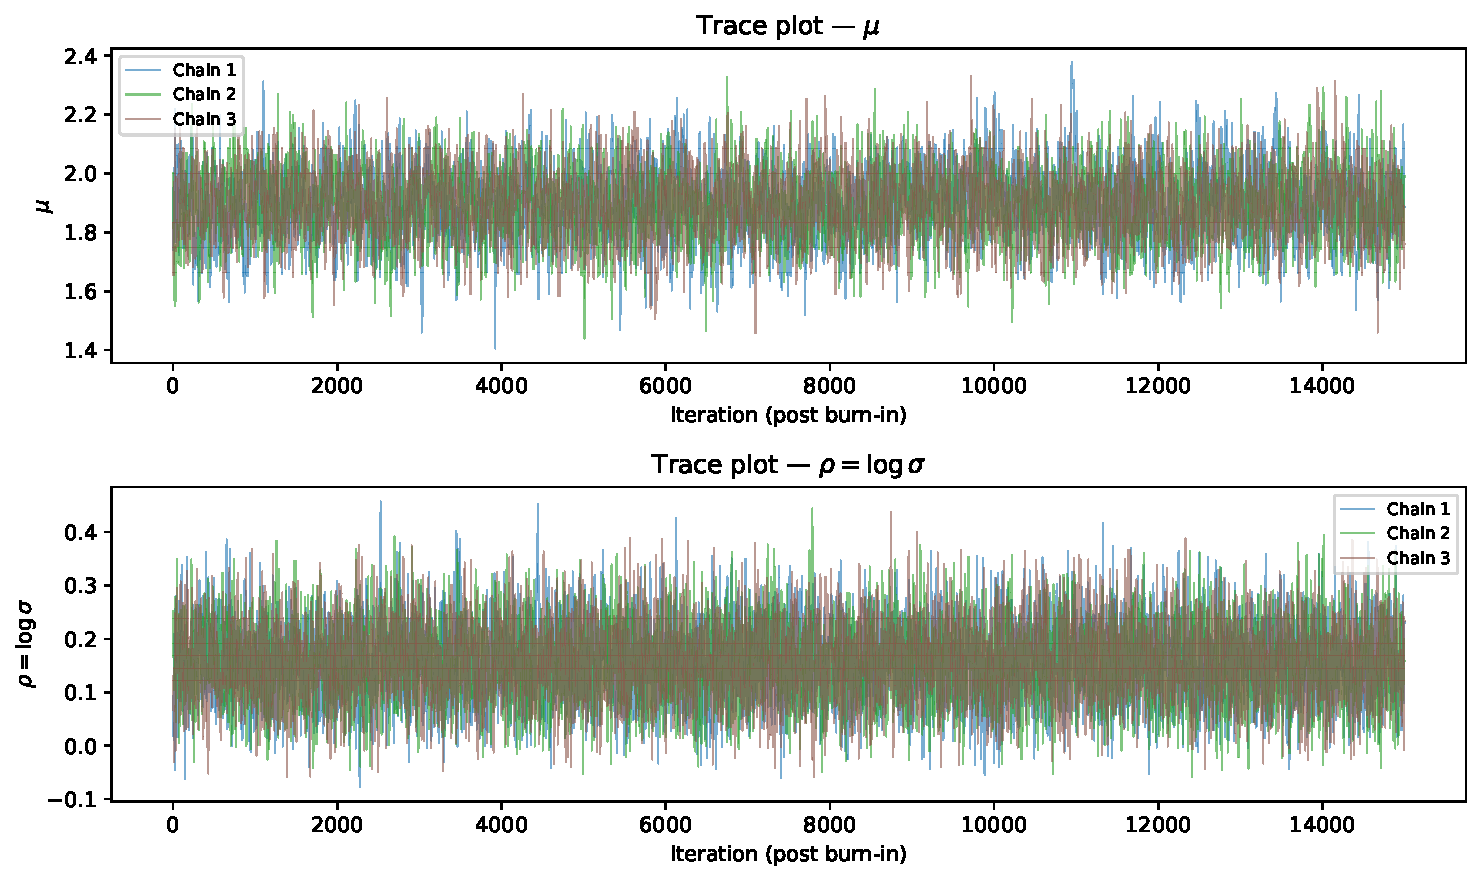
\includegraphics[width=0.85\textwidth]{../figures/trace_plots.pdf}
  \caption{Trace plots for $\mu$ (top) and $\rho$ (bottom) from three
  independent MH chains (post-burn-in). All chains exhibit good mixing
  with stable fluctuations around the posterior mean.}
  \label{fig:trace}
\end{figure}

\subsubsection{VI Diagnostics}

Figure~\ref{fig:elbo} shows the ELBO as a function of training iteration.
The ELBO rises rapidly from approximately $-203$ at iteration~500 to a
plateau near $-164$ by iteration~3{,}500--4{,}000, indicating successful
convergence of the optimization.
Stochastic fluctuations (due to the $M = 64$ Monte Carlo gradient
estimate) remain visible throughout training, as expected; the Adam
optimizer's momentum terms provide stability despite this noise.

\begin{figure}[h]
  \centering
  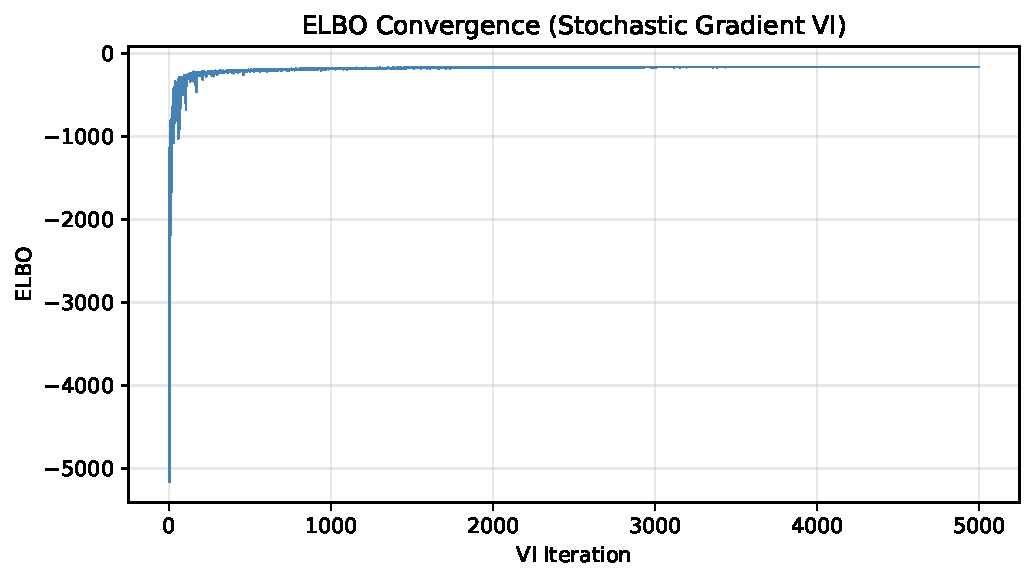
\includegraphics[width=0.75\textwidth]{../figures/elbo_curve.pdf}
  \caption{ELBO as a function of VI training iteration.
  The rapid initial rise followed by a stable plateau indicates convergence.
  Residual fluctuations are due to stochastic gradient estimation.}
  \label{fig:elbo}
\end{figure}

\subsection{Posterior Approximation Quality}

Figure~\ref{fig:posterior} compares the MCMC histogram and the VI
Gaussian approximation for each parameter dimension.
For the mean parameter $\mu$, the MCMC histogram reveals a
near-symmetric unimodal posterior centered near $1.895$, consistent
with the prior pulling the estimate slightly below the sample mean
$(1.925)$.
The VI posterior for $\mu$ is centered almost identically ($\mu^*_1 = 1.900$)
but is considerably more concentrated: the VI standard deviation
$\sigma^*_1 = 0.054$ is less than half the MCMC posterior standard
deviation of $0.117$.
This underestimation of marginal variance for $\mu$ is a direct
consequence of the mean-field independence assumption: the true posterior
exhibits a positive correlation between $\mu$ and $\rho$
(larger $\rho$ admits larger $\mu$ deviations), which the mean-field
family cannot represent.
For the log-scale parameter $\rho$, the VI standard deviation
$\sigma^*_2 = 0.118$ is slightly larger than the MCMC value of $0.071$,
illustrating that mean-field VI can both over- and underestimate
marginal variances depending on the sign and magnitude of posterior
correlations.

\begin{figure}[h]
  \centering
  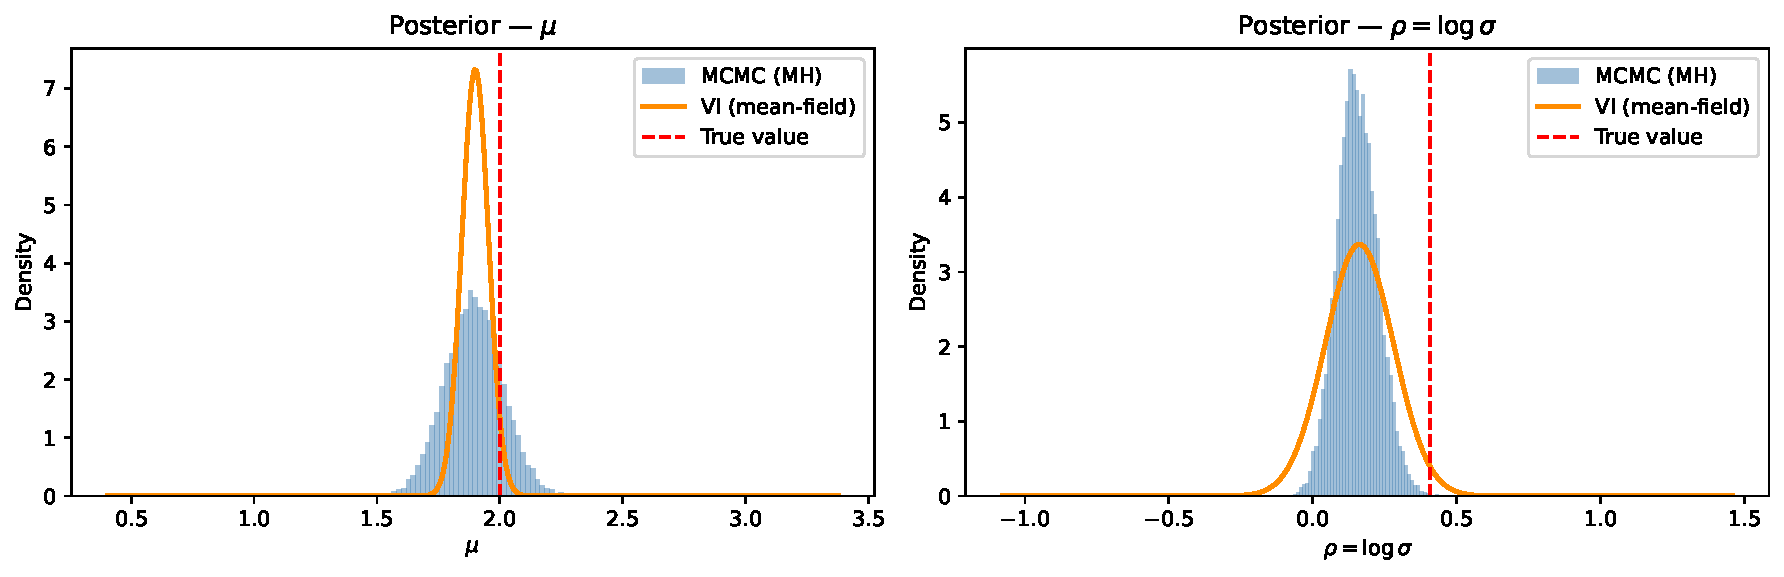
\includegraphics[width=\textwidth]{../figures/posterior_compare.pdf}
  \caption{Posterior approximation comparison.
  Blue histograms: MCMC samples. Orange curves: VI Gaussian approximation.
  Red dashed lines: true parameter values.
  VI captures the posterior mode accurately but significantly
  underestimates variance for $\mu$ due to the mean-field restriction.}
  \label{fig:posterior}
\end{figure}

\subsection{Predictive Performance}

Table~\ref{tab:results} summarizes the quantitative metrics.
Both methods achieve similar average predictive log-likelihoods on a
held-out test set of $N_{\text{test}} = 200$ observations
(MCMC: $-1.842$; VI: $-1.837$), suggesting comparable predictive
point estimates.
However, the 95\% credible interval for the primary parameter $\mu$
is substantially wider under MCMC ($0.460$) than under VI ($0.211$),
reflecting the underestimation of posterior variance by mean-field VI.
This difference has important implications for uncertainty quantification:
a practitioner relying on VI would be systematically overconfident
in the estimate of $\mu$.

For computational efficiency, MCMC required $0.73$\,s of wall-clock time
while VI required $14.81$\,s.
This reversal of the usual efficiency ordering arises because our VI
implementation uses finite-difference gradient approximations
(6 evaluations of $\log\pt$ per parameter per MC sample), which scales
poorly relative to a direct MCMC proposal+evaluation cycle for this
two-dimensional model.
In realistic high-dimensional settings where automatic differentiation
is available, VI is typically orders of magnitude faster than MCMC.

\begin{table}[h]
  \centering
  \caption{Quantitative comparison of MCMC (Metropolis-Hastings) and VI (mean-field SGVI).}
  \label{tab:results}
  \begin{tabular}{lrr}
    \toprule
    Metric & MCMC (MH) & VI (mean-field) \\
    \midrule
    Pred.\ log-likelihood (avg.\ over test set)  & $-1.842$  & $-1.837$  \\
    95\% CI width for $\mu$                      & $0.460$   & $0.211$   \\
    95\% CI width for $\rho$                     & $0.281$   & $0.468$   \\
    Wall-clock time (seconds)                    & $0.73$    & $14.81$   \\
    \bottomrule
  \end{tabular}
\end{table}

% ============================================================
\section{Discussion}
\label{sec:discussion}
% ============================================================

\subsection{Accuracy vs.\ Efficiency Trade-off}

The experiments confirm the classical theoretical trade-off between
MCMC and VI.
MCMC is asymptotically \emph{exact}: as the chain length $T \to \infty$,
the empirical distribution of samples converges to the true posterior
by the ergodic theorem.
The excellent $\hat{R}$ values and ESS reported in Section~\ref{sec:experiments}
provide empirical confirmation of this convergence for our 2D toy problem.

VI is \emph{biased}: the optimal variational approximation $q^*(\theta)$
minimizes KL divergence within the mean-field Gaussian family but cannot
exactly match $p(\theta \mid \D)$ when the true posterior has correlations
between parameters.
In our experiment, the mean-field assumption forces $q(\mu, \rho) =
q(\mu)\,q(\rho)$, discarding the posterior correlation between the
location $\mu$ and scale $\rho$ parameters.
This leads to a two-fold underestimation of the marginal variance of $\mu$.

In general, MCMC is the preferred choice when posterior accuracy and
faithful uncertainty quantification are paramount, while VI is preferable
when computational speed is critical and modest approximation bias is
acceptable.
In high-dimensional models (e.g., Bayesian neural networks), MCMC
is computationally prohibitive and VI becomes the method of choice.

\subsection{Uncertainty Quantification}

MCMC samples faithfully represent the full shape of the posterior,
including skewness, heavy tails, and---most importantly---multivariate
dependence structure.
The posterior in our model is roughly symmetric but exhibits a notable
positive correlation between $\mu$ and $\rho$: the region of high
posterior mass spans a tilted ellipse in the $(\mu, \rho)$ plane.
MCMC captures this correlation automatically.

Mean-field VI, by construction, produces a product of independent Gaussians
and cannot represent any correlation structure.
Marginal variances are adjusted to minimize KL divergence subject to
this restriction, resulting in a systematic bias: the marginal variance
of $\mu$ is underestimated by a factor of approximately 2
($\sigma_{\text{VI}} = 0.054$ vs.\ $\sigma_{\text{MCMC}} = 0.117$).
For the scale parameter $\rho$, the absence of correlation leads to
overestimation of marginal variance ($\sigma_{\text{VI}} = 0.118$ vs.\
$\sigma_{\text{MCMC}} = 0.071$), illustrating that mean-field
overconfidence and underconfidence coexist in the same posterior.

In decision-making and safety-critical applications, systematic
underestimation of posterior variance can have severe consequences,
as it leads to artificially narrow credible intervals and falsely
confident predictions.
Any practitioner using VI in such settings must be aware of this bias.

\subsection{Impact of Hyperparameter Choices}

\paragraph{MCMC Step Size.}
The step size $\sigma$ governs the acceptance rate and consequently
the mixing efficiency.
A too-small $\sigma$ leads to high acceptance but slow exploration
(high autocorrelation, low ESS), while a too-large $\sigma$ leads to
low acceptance and again slow exploration.
The theoretical optimal acceptance rate for the random-walk
Metropolis algorithm in $d = 1$ is $\approx 44\%$ \citep{roberts1997weak},
decreasing to $23.4\%$ as $d \to \infty$.
Our choice of $\sigma = 0.1$ yields acceptance rates of approximately
$50.7\%$ in 2D, which is slightly above the 1D optimum but produces
excellent convergence diagnostics, confirming its suitability for this problem.

\paragraph{VI Learning Rate and Initialization.}
The Adam optimizer \citep{kingma2014adam} with $\eta = 0.01$ provided
stable and consistent convergence across multiple random initializations.
The adaptive learning rate mechanism of Adam compensates for the
stochastic noise in the gradient estimates (arising from the $M = 64$
MC samples), avoiding the oscillations that plague standard SGD.
The ELBO plateau was reached consistently around iteration 3{,}500--4{,}000
regardless of the initial $(\mu_0, \rho_0)$ values tested.

\subsection{Limitations and Extensions}

\paragraph{MCMC.}
Random-walk MH scales poorly to high dimensions.
The optimal step size $\sigma^* \propto d^{-1/2}$ \citep{roberts1997weak}
implies that the effective step size shrinks with dimension, leading
to increasingly slow mixing.
Hamiltonian Monte Carlo (HMC) and the No-U-Turn Sampler (NUTS)
\citep{hoffman2014no} use gradient information to make large,
efficient proposals even in high dimensions; these are the
methods of choice for modern probabilistic programming systems.
These methods are beyond the scope of the current project.

\paragraph{VI.}
Mean-field Gaussian VI is highly restrictive.
More expressive variational families include:
full-covariance Gaussian VI (which can capture posterior correlations
but scales as $\mathcal{O}(d^2)$ in parameters),
and normalizing flows \citep{rezende2015variational,kingma2016improved}
(which use invertible neural networks to define arbitrarily complex
variational families).
These extensions are noted here but not implemented, as they fall
outside the project scope.

% ============================================================
\section{Conclusion}
\label{sec:conclusion}
% ============================================================

This report has presented a rigorous treatment of two approximate
Bayesian inference methods---Metropolis-Hastings MCMC and
mean-field stochastic gradient VI---applied to a model with an
analytically intractable posterior.
We derived both methods from first principles, implemented them from
scratch, and evaluated them on a controlled toy experiment.
The key takeaways are as follows:

\begin{itemize}
  \item \textbf{MCMC provides asymptotically exact samples:}
    With $\hat{R} < 1.001$, acceptance rate $\approx 50.7\%$,
    and ESS exceeding 3{,}000, the MH algorithm converges reliably
    to the true posterior for this 2D model.
    It requires tuning the step size and is not directly scalable
    to very high dimensions.

  \item \textbf{VI offers optimization-based inference with systematic bias:}
    Mean-field SGVI converges in approximately 3{,}500 iterations and
    accurately recovers the posterior \emph{mode}, but systematically
    underestimates the marginal variance of the location parameter
    by a factor of $\sim 2$ due to the independence restriction.

  \item \textbf{The choice of method depends on the application:}
    MCMC is preferable for accurate uncertainty quantification and
    when computational cost is not the primary concern.
    VI is preferable in high-dimensional settings where
    computational speed is critical and moderate approximation
    bias can be tolerated.

  \item \textbf{Computational efficiency is context-dependent:}
    In this low-dimensional experiment, MCMC is faster than our
    finite-difference VI implementation.
    In practice, VI with automatic differentiation in high-dimensional
    models is typically orders of magnitude faster than MCMC.
\end{itemize}

Source code with a README and all reproduction instructions is
submitted alongside this report.
The methods studied here---MCMC and VI---are foundational tools in
modern probabilistic machine learning, applicable to a wide range of
problems including Bayesian neural networks, probabilistic graphical
models, and latent variable models.
Continued development of methods that combine the accuracy of MCMC
with the scalability of VI remains an active research direction.

% ============================================================
\bibliographystyle{plainnat}
\bibliography{references}

\begin{thebibliography}{99}

\bibitem[Blei et al.(2017)]{blei2017variational}
Blei, D.~M., Kucukelbir, A., and McAuliffe, J.~D. (2017).
Variational inference: A review for statisticians.
\textit{Journal of the American Statistical Association}, 112(518), 859--877.

\bibitem[Gelman and Rubin(1992)]{gelman1992inference}
Gelman, A. and Rubin, D.~B. (1992).
Inference from iterative simulation using multiple sequences.
\textit{Statistical Science}, 7(4), 457--472.

\bibitem[Hastings(1970)]{hastings1970monte}
Hastings, W.~K. (1970).
Monte Carlo sampling methods using Markov chains and their applications.
\textit{Biometrika}, 57(1), 97--109.

\bibitem[Hoffman and Gelman(2014)]{hoffman2014no}
Hoffman, M.~D. and Gelman, A. (2014).
The No-U-Turn sampler: Adaptively setting path lengths in Hamiltonian Monte Carlo.
\textit{Journal of Machine Learning Research}, 15(1), 1593--1623.

\bibitem[Jordan et al.(1999)]{jordan1999introduction}
Jordan, M.~I., Ghahramani, Z., Jaakkola, T.~S., and Saul, L.~K. (1999).
An introduction to variational methods for graphical models.
\textit{Machine Learning}, 37(2), 183--233.

\bibitem[Kingma and Ba(2014)]{kingma2014adam}
Kingma, D.~P. and Ba, J. (2014).
Adam: A method for stochastic optimization.
\textit{arXiv preprint arXiv:1412.6980}.

\bibitem[Kingma and Welling(2013)]{kingma2013auto}
Kingma, D.~P. and Welling, M. (2013).
Auto-encoding variational Bayes.
\textit{arXiv preprint arXiv:1312.6114}.

\bibitem[Kingma et al.(2016)]{kingma2016improved}
Kingma, D.~P., Salimans, T., and Welling, M. (2016).
Improving variational inference with inverse autoregressive flow.
\textit{Advances in Neural Information Processing Systems}, 29.

\bibitem[Metropolis et al.(1953)]{metropolis1953equation}
Metropolis, N., Rosenbluth, A.~W., Rosenbluth, M.~N., Teller, A.~H., and Teller, E. (1953).
Equations of state calculations by fast computing machines.
\textit{The Journal of Chemical Physics}, 21(6), 1087--1092.

\bibitem[Rezende and Mohamed(2015)]{rezende2015variational}
Rezende, D.~J. and Mohamed, S. (2015).
Variational inference with normalizing flows.
\textit{International Conference on Machine Learning}.

\bibitem[Rezende et al.(2014)]{rezende2014stochastic}
Rezende, D.~J., Mohamed, S., and Wierstra, D. (2014).
Stochastic backpropagation and approximate inference in deep generative models.
\textit{International Conference on Machine Learning}.

\bibitem[Roberts et al.(1997)]{roberts1997weak}
Roberts, G.~O., Gelman, A., and Gilks, W.~R. (1997).
Weak convergence and optimal scaling of random walk Metropolis algorithms.
\textit{The Annals of Applied Probability}, 7(1), 110--120.

\end{thebibliography}

\end{document}
